% !Mode:: "TeX:UTF-8"

\chapter{绪论}

\section{课题研究的背景和意义}

在软件的生命周期中,持续的代码维护是保证系统长期稳定发展的关键环节。研究表明,软件系统的维护成本在长期的项目维护预算中占据了60\%至80\%的比例\cite{2012Maintenance}。维护过程中,开发人员不仅要对现有代码进行修改,还要确保新增功能或修复的缺陷不会影响系统原有的稳定性和性能。为了确保软件质量,维护工作通常依赖于系统的回归测试和代码审查。具体来说,标准的代码开发流程通常包括以下三个主要步骤,如图1-1所示。

\begin{figure}[h]
\centering
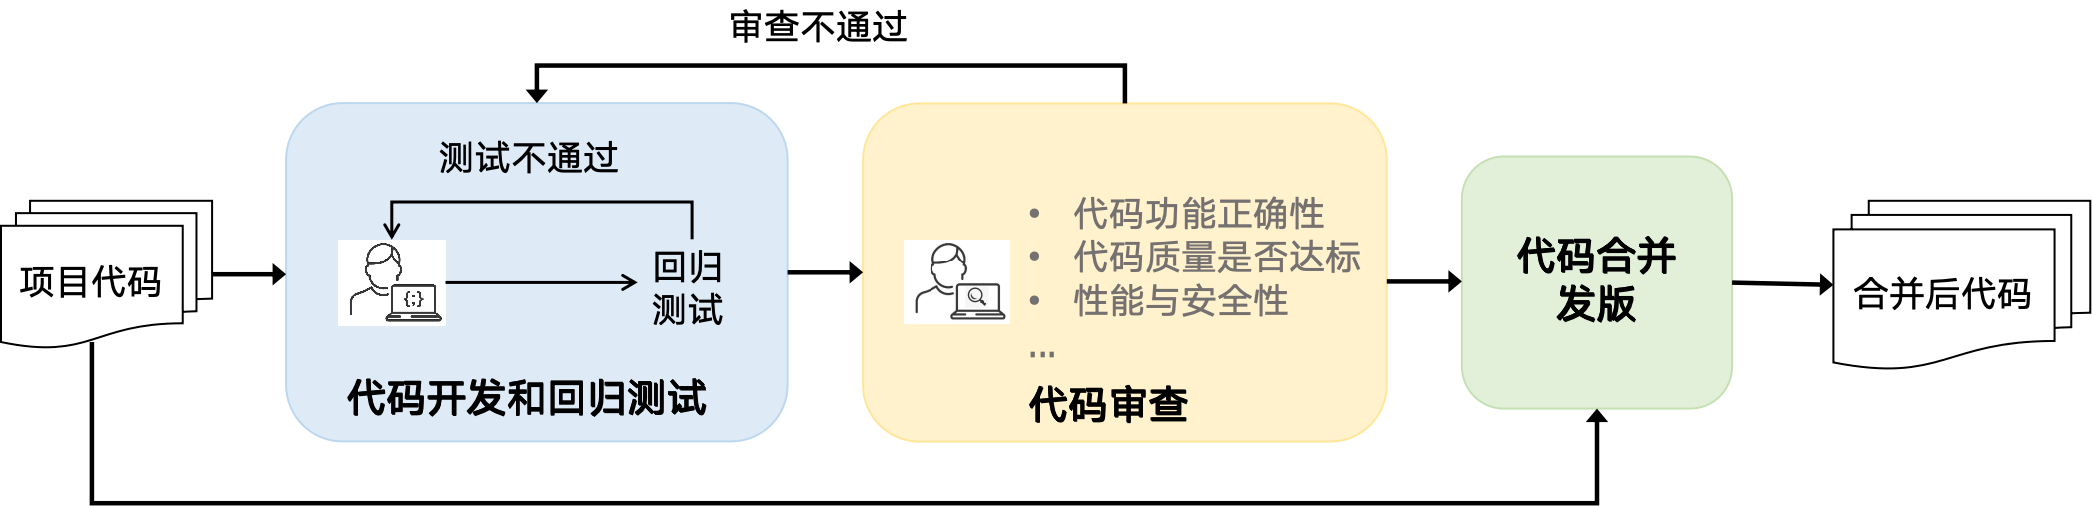
\includegraphics[width = 1.0\textwidth]{代码开发流程.png}
\caption{标准代码开发流程}
\end{figure}

(1)代码开发与回归测试:开发人员在对项目代码进行修改后,首先对修改部分进行回归测试,验证新功能是否符合需求并避免新缺陷的引入。

(2)代码审查:当测试通过后,代码将提交给审查人员进行审查。代码审查不仅仅是对代码逻辑正确性的检查,更是一个确保代码质量的重要环节。通过代码审查可以识别潜在的错误,提出代码优化建议,并统一开发团队的编码风格,从而提高代码的可维护性和可靠性。

(3)代码合并:审查通过后,修改的代码可以与原始项目进行合并,进入下一个开发周期。在此过程中,确保代码的正确性和稳定性是至关重要的,避免因合并而引入新的问题。

在代码审查环节中,代码质量评估是确保软件项目高效、可维护和可扩展的基础手段之一。随着软件系统的规模和复杂性的不断增长,代码质量直接影响到系统的稳定性、可维护性以及开发过程中的效率。良好的代码质量不仅有助于减少潜在的缺陷,提高软件的可靠性,还能在团队协作中提高开发效率,降低维护成本。但是传统的依赖经验丰富的专家进行代码审查,在面对日益复杂化的系统结构时,显得力不从心\cite{2016Microservices}。因此,研究自动化的代码质量评估方法,成为了软件工程领域的重要研究课题。

对软件项目的持续开发和维护过程中,代码变更不可避免。在代码修改、功能新增或缺陷修复的过程中,变更可能会对现有代码的质量和系统的整体结构产生深远的影响。变更影响分析(Change Impact Analysis,CIA)方法作为一种有效的工具,能够在代码变更发生时预测变更可能带来的影响,帮助开发人员更好地理解变更对其他模块或代码的潜在影响,从而做出更加合理的设计和优化决策。变更影响分析不仅能够避免意外的质量下降,还能帮助开发者在变更过程中有效地识别和规避高风险区域,确保代码质量不会因变更而受到负面影响。

对于大型软件系统,代码变更影响分析更显得尤为关键。随着软件规模的不断扩大和开发团队的不断扩展,系统往往融合了不同开发者的个性化风格。与此同时,系统的模块化设计原则可能在逐步演化过程中被复杂和庞大的代码结构所淹没,导致系统变得更加难以维护。这种情况下,精准地识别变更后受影响的代码,对于系统的持续维护具有至关重要的意义。因此,从代码变更影响分析的角度出发,不仅能深入理解代码变更对系统整体和各个子模块的潜在影响,还能够提高维护项目的效率\cite{2022An}。这种方法为软件系统的维护和升级提供了一种更为科学和系统的解决策略,有助于实现软件质量的持续提升和维护成本的有效控制。

本文面向代码质量评估,通过静态分析方法对代码项目进行代码度量提取和缺陷检测,并检测代码变更影响分析入手进行方法研究,将最终的分析结果以代码审查图的形式展示,帮助开发者和审查人员更直观地理解整个项目的质量情况和代码变更影响情况,优化项目的持续维护过程,为维护项目代码提供更有效的保障。

\section{国内外研究现状及分析}


\subsection{代码质量研究主题的国内外研究现状}

软件质量与软件的稳定性、可靠性、健壮性和可维护性等关键特性密切相关,是衡量软件性能和可靠性等指标的重要标准。作为软件质量的重要组成部分,代码质量在整体软件质量中占据着至关重要的地位,直接影响着软件系统的长期可用性与可维护性。根据近年来对代码质量研究的广泛性进行排名\cite{NUNEZVARELA2017164},代码质量研究主题主要可以分为以下几种,

(1)代码缺陷

代码缺陷是研究最广泛的代码质量主题。相近地,代码漏洞、代码故障等也属于代码缺陷的范畴。软件代码中往往存在大量隐藏的缺陷,这些缺陷可能源于开发人员的疏忽、软件固有的逻辑漏洞或开发语言安全性的脆弱性,如果不进行及时的处理,这些问题可能引发安全漏洞,对软件的安全造成影响。在此主题中,缺陷检测和预测是最主要的研究目的。

目前的研究方法主要分为三种,首先是传统的基于静态分析的方法,如基于代码相似度的检测器\cite{Sheneamer2018A,2014A}或基于模式的检测器\cite{2012Mitigating,2017IDE,2016How}。这种检测方法基于一系列预定义的规则、模式或静态模型进行检查,但是通常会产生较高的误报,检测的效果取决于预先定义的规则或模式的质量。其次是基于机器学习的方法。该种方法通过文本分析等方法提取代码特征,结合分类器,如决策树、支持向量机等机器学习技术\cite{2017Assessment,2018A,2020The},在大型数据集上进行预测。随着深度学习技术的发展,逐渐出现了基于深度学习技术的缺陷或漏洞预测方法,这种检测方法主要分为两步,首先通过代码表示学习方法,将代码表示为词嵌入、图表示或序列表示,利用神经网络捕捉代码语义和结构特征。通过端到端的深度学习模型直接从原始代码或中间表示中学习缺陷模式,训练模型后,直接对代码进行缺陷预测。


(2)代码复杂度

代码复杂度也是代码质量研究领域的重要主题之一。在Alberto等人\cite{NUNEZVARELA2017164}的研究中统计,代码复杂度在代码质量的主题中研究数量排在第二位。研究方法可分为以下三种,一是基于传统度量指标的研究,这类研究通常是对经典复杂度度量的扩展,如在传统的度量标准,如圈复杂度、Halstead复杂度等的基础上,结合新型指标进行复杂度评估。二是基于复杂网络来进行研究\cite{2015Exploring, 2012A},这类研究中通常将代码转化为图数据,如抽象语法树、调用图、控制流图、数据流图等,通过分析图结构的复杂性,捕捉代码逻辑的复杂程度。三是基于认知复杂度的方法,认知复杂度衡量执行任务所需的人类努力\cite{2012Framework, 2012Asuite},是由Shao和Wang\cite{2010Assessing}等人提出的认知指标的重要组成部分,这些度量标准与任何特定的编程范例都没有关联,但是可以从人因工程视角评估代码的认知复杂性,研究代码结构(如嵌套、条件分支)对开发者理解负担的影响,从而衡量代码的复杂性。


(3)代码内聚度和耦合性

内聚度和耦合性是软件设计中的核心指标,二者之间往往存在着此消彼长的关系,它们的平衡直接影响系统的质量与可维护性。高内聚度表示模块内部功能集中且相关性强,有助于提高代码的可读性和复用性,降低修改时的风险;低耦合性则强调模块间独立性,减少了相互依赖导致的连锁反应,使得系统更易于扩展和测试。二者共同作用,构成了高质量、易维护的软件架构的基础。

近年来对于内聚度的研究大多是从不同的角度提出新的度量标准,有部分研究是对传统度量指标的改进。Chen 等人 \cite{陈振强2003} 提出了基于程序依赖性分析的类内聚度度量方法,该方法从属性与属性、属性与方法、方法与方法之间的依赖关系出发,全面分析类的内聚性。该方法不仅支持单独度量类的内聚度,还可以结合多种度量方式进行综合评估。研究表明,该方法符合 Briand \cite{1997Property} 提出的优良内聚度度量标准的四项基本要求。QU\cite{QU2015193}提出了两个新的类内聚度量MCC(Method Community Cohesion)和MCEC(Method Community Entropy Cohesion),这两种指标基于类中方法在不同社区间的分布,反映类的内聚程度。研究表明,这两种指标可以提供现有类内聚指标所未反映的额外且有用的信息。

同内聚度类似,对于耦合性的研究大部分也是对传统度量指标的改进。Ma等人\cite{马健2018}参考 UML 中类图之间的关系,对 CBO (Coupling Between Object Classes)度量指标进行了改进,并使用一组形式化评估软件质量性质的定理进行评估, 以 JUnit 和 JEdit 为研究对象,对提出度量框架的关联、依赖、泛化关系进行度量研究。结果分析表明,改进后的指标可以较准确地反映面向对象设计中的耦合关系。

除此之外,还包括代码变更、代码可重用性、代码可读性、代码性能和代码安全性等研究主题。

\subsection{代码质量度量的国内外研究现状}

根据不同的研究主题,演化出了很多代码度量套件,这些度量套件被广泛应用于各种软件项目上,在软件生命周期的各个环节(例如,开发、测试、重构)上被使用,以评估软件的整体质量。为了满足不同的度量需求,多年来,人们提出、研究和验证了许多来自不同编程范型的源代码度量,并不断提出新的度量和研究。研究发现\cite{Ardito2020},近年来使用最广泛的是Chidamber and Kemerer套件(CK套件)和Li and Henry(L&H)套件。


\begin{table}[htbp]
\caption{CK套件核心指标}
\vspace{0.5em}\centering\wuhao
\begin{tabular}{ccp{7.5cm}}
\toprule
度量 & 全称 & 描述 \\
\midrule
WMC & Weighted Methods per Class & 类中的方法的复杂性,复杂性可以通过方法数量或具体的计算方式(如方法的圈复杂度)来衡量 \\
DIT & Depth of Inheritance Tree & 类在继承树中的深度 \\
NOC & Number of Children & 一个类直接子类的数量 \\
CBO & Coupling Between Object Classes & 类与其他类之间的耦合关系数量  \\
RFC & Response for a Class & 类能够响应的所有方法的数量,包括其直接定义的方法和调用的其他类的方法  \\
LCOM & Lack of Cohesion in Methods & 类中方法间缺乏内聚性的程度  \\
\bottomrule
\end{tabular}
\end{table}

CK套件主要是针对面向对象语言设计的度量套件,所含度量与其具体含义如表1-1中所示。CK套件中共有六个核心度量,侧重点各有不同,其中WMC用于衡量类的复杂性。如果值较高,说明类可能过于复杂,难以维护。DIT用于衡量类继承层次的复杂性。较大的DIT值表明更深的继承层次,增加了设计复杂性。NOC计算了一个类的直接子类的数量,衡量了类的影响范围,NOC值较高可能表明父类的职责过于泛化。CBO衡量了类间的依赖性,如果值较高,表示类之间耦合较强,模块化和重用性可能会较低。RFC衡量类的复杂性和可能的行为范围,RFC值较高可能表明类的行为过于复杂。LCOM衡量类内部方法和字段的相关性,如果值较高,说明类可能职责分散,应考虑拆分或重构优化。CK套件提供了一种系统化的方法来评估软件质量,能够帮助开发人员识别潜在问题,改进代码可维护性和可重用性。虽然CK套件主要是应用于面向对象语言的,但是也可应用于面向过程语言,只是需要根据具体场景调整权重和解释。

L\&H套件是由Li和Henry等人提出\cite{1993Object}的,用于评估程序的复杂度、维护性以及开发成本等的度量套件。L&H套件中有一部分度量和CK套件是一样的,除此之外,还有另外五个核心指标,具体度量名称和含义见表1-2。

\begin{table}[htbp]
\caption{L\&H套件核心指标}
\vspace{0.5em}\centering\wuhao
\begin{tabular}{ccp{8cm}}
\toprule
度量 & 全称 & 描述 \\
\midrule
DAC & Weighted Methods per Class & 类之间通过抽象数据类型(Abstract Data Type)进行交互的程度 \\
MPC & Message Passing Coupling & 类之间通过方法调用进行通信的频率 \\
NOM & Number of Methods & 类中所有方法(包括继承和自定义方法)的数量 \\
SIZE2 & Second Order Size Metric & 通常用类的属性数和方法数的平方和表示  \\
SLOC & Source Lines of Code & 源代码行数  \\
\bottomrule
\end{tabular}
\end{table}

其中,较高的 DAC和MPC 值表示类对其他类的依赖程度较高,可能导致耦合度增加。较高的NOM和SIZE2 可能表明类的职责过多,过于复杂,难以理解和维护。较高的 SLOC 值表示代码较为冗长,可能需要优化。


\subsection{代码变更影响分析方法}

变更影响分析(Change Impact Analysis,CIA)是软件工程中用于分析代码变更对系统其他部分可能产生的影响的一种技术。研究表明,代码变更对代码质量的影响在大规模软件中尤为显著。Wenchen 等人的研究指出\cite{2013Large},在大型系统中,每个版本的补丁可能影响约 2\% 的代码,这对全面的程序回归测试提出了巨大挑战。因此,针对受变更影响的代码区域进行精确测试则是一种既高效又安全的测试方案。此方法不仅能够有效降低时间和资源成本,还能在不牺牲系统质量的前提下,减少因回归测试覆盖不足而引发的潜在漏洞或故障风险。这一策略强调了将代码变更范围与回归测试策略精细化结合的重要性,为提升软件开发和维护阶段的代码质量提供了有力支持。

自Arnold等人\cite{Arnold1996}提出变更影响分析的概念以来,它一直是代码审查的重要组成部分之一。该方法支持用户在代码变更之前对其影响进行分析,从而估计变更可能造成的负面影响,其优势可总结如下:(1)能提升代码的稳定性和可靠性。通过分析代码变更对相关模块的影响,开发者可以识别潜在的故障或不一致之处,在变更合入前发现问题,避免引入新的缺陷,从而提高系统的稳定性和可靠性。(2)有助于模块化设计和低耦合。变更影响分析能够反映出代码模块之间的依赖关系和耦合程度,通过减少不必要的耦合,增强代码的模块化特性,从而提升代码的可维护性和可扩展性。(3)有助于代码质量的提高。通过变更影响分析能够记录变更过程中的风险评估和解决措施,满足质量保证和审查的需求,提高软件开发过程的透明性和可追踪性。(4)有助于开发团队协作。变更影响分析为团队提供了清晰的变更范围和影响信息,便于团队成员之间协调工作,减少因沟通不足导致的重复工作或冲突,同时提高代码可读性,有助于开发团队更快速地理解系统,减少后期维护成本。

目前变更影响分析的相关技术主要分为静态分析和动态分析两类。

(1)静态变更影响分析方法

静态分析方法因其具有高覆盖率和高安全性的优势,广泛应用于对安全性要求较高的软件回归测试中。这类方法通过基于程序的中间表示(如控制流图、调用图等)来进行分析。在静态分析方法中,过程内分析方法通常依赖于程序切片、控制流和数据流等技术\cite{2004Efficient,1991Using},而过程间的影响分析则主要通过计算调用图或系统依赖图的传递闭包来揭示不同模块之间的依赖关系\cite{JitenderKumarChhabra2018Improved, 2011An, 2013Analyzing}。

Schrettner等人\cite{Department2013Impact}提出了一种创新的静态执行后关系(Static Execute After, SEA)方法,这是一种计算高效且足够精确的程序关系,表示代码之间的运行顺序紧密相连的情况,可以作为变更影响分析的基础。SEA的提出为程序分析提供了新的视角,其实验结果表明,通过SEA计算得到的影响关系能够发现大量的实际影响关系,显著提高了静态分析的准确性和实用性。

Sun等人\cite{5676283}提出了将变更类型与影响机制相结合的变更影响分析方法。他们认为不同类型的软件变更通常会带来不同的影响机制,因此需要根据变更的具体类型来制定相应的影响分析策略。此外,他们还指出,影响关系的精确度与初始影响关系的精确度密切相关,初始影响关系越精确,基于其计算得到的最终影响关系也会更为准确。这一发现为改进影响分析技术提供了新的思路,强调了初始数据质量对最终分析结果的重要性。

近年来,随着软件系统复杂度的增加,单一的变更影响分析方法已经难以满足高效性和准确性的双重需求。因此,研究人员提出了混合变更影响分析(CIA)技术,通过将多种CIA方法结合起来,以提高变更影响分析的准确性和健壮性\cite{2021Improving}。混合CIA技术的核心思想是将不同方法的优势互补,从而弥补单一方法的不足。研究表明,结合至少两种CIA技术的混合策略能够显著提高性能,且相比于基线技术,混合CIA方法始终表现出更好的性能改进。这一进展为变更影响分析提供了新的解决方案,尤其适用于大型复杂系统的影响分析任务。

(2)动态变更影响分析方法

尽管静态影响分析在软件工程中因其较高的覆盖率和较好的安全性而被广泛应用,但其分析结果往往存在精确性不足的问题。这是因为静态分析主要依赖程序的中间表示(如控制流图、调用图等)进行推理,而这些模型无法捕捉程序在运行过程中可能出现的实际行为。为了弥补这一不足,一些研究者转向动态影响分析。与静态分析不同,动态影响分析是在程序运行时收集实际执行信息,并基于这些运行时数据计算程序中各个部分的影响关系。尽管动态分析通常能够提供更为精确的结果,但其成本较高,而且在面对复杂的系统时,无法确保分析结果的完全安全性。

尤其是在面向对象编程的系统中,由于程序实体之间的依赖关系较为复杂且难以静态建模,动态分析的结果有时会产生不精确性的影响。为了提高动态分析的精确性,Huang等人\cite{2007Precise}提出了一种专门针对面向对象程序的精确动态变更影响分析方法。该方法结合了面向对象编程的特性,能够更加准确地确定程序实体之间的实际影响关系。同时,Huang等人通过排除与变更对象无关的程序部分,显著减少了分析的规模,从而提升了分析的效率和精度。

在动态变更影响分析的精确性和可靠性方面,Cai等人\cite{2015Acom,2014Estimating}进行了深入研究。他们提出了一种实验方法,首先通过敏感性分析来评估变更影响分析的准确性,然后通过实施软件变更并观察这些变更的实际影响,进一步分析其精确度和召回率。这一方法为动态影响分析技术的有效性提供了重要的实证依据,并揭示了在实际应用中可能遇到的挑战。此外,Cai等人还提出了针对分布式系统的动态影响分析方法——DISTIA\cite{2016DistIA}。该方法通过对分布式系统中各个执行事件进行部分排序,并根据这些排序推断事件之间的因果关系,同时结合消息传递的语义预测影响在不同进程边界内外的传播情况,有效地解决了分布式系统中的影响传播问题,为分布式软件的动态影响分析提供了新的技术路径。

(3)其他代码变更影响分析方法

除了上述静态和动态分析方法外,另一些研究并未直接关注软件本身,而是将关注点转向软件变更的历史库\cite{2011An, Markus2017Supporting, 2008Mining, 2014Impact, 2016Generalizing}。这些研究认为,软件变更历史记录中包含了大量与程序及其演化相关的信息,分析和挖掘这些信息能够帮助识别和预测变更对软件系统的潜在影响。这些依赖关系和变更模式可以通过数据挖掘方法、信息检索技术以及机器学习等手段进行挖掘和分析,从而为变更影响分析提供新的视角和方法。

Gethers等人\cite{2011An}采用了信息检索、动态分析和数据挖掘方法,基于历史源代码提交记录改进了变更影响方法的生成技术。通过分析过去的源代码提交,研究者能够更好地识别变更和其他程序部分之间的潜在依赖关系,从而生成更加精确的变更影响集。这一方法突出了历史数据的重要性,利用现有的变更历史信息来为未来的变更影响分析提供依据,从而提升了分析的准确性和效率。

Zanjani等人\cite{2014Impact}提出了一种结合交互历史和提交历史的方法来分析源代码变更请求。他们的创新之处在于将信息检索、机器学习和轻量级源代码分析相结合,通过构建源代码实体的语料库,来提高变更影响分析的精确度。当给定一个变更请求的文本描述时,该语料库可以被查询,并返回一个按相关性排序的最可能发生变更的源代码实体列表。这种方法能够通过历史变更请求的文本描述,准确预测哪些源代码实体可能受到影响,为开发人员提供有效的决策支持。

Rolfsnes等人\cite{2016Generalizing}致力于改进现有的耦合分析算法,尤其是在软件变更的上下文中。TARMAQ算法是他们提出的一种新型算法,在性能上明显优于ROSE\cite{2005Mining}和SVD等传统算法。TARMAQ通过挖掘代码库中的耦合关系,能够更精确地揭示源代码之间的依赖和关联,从而提高了变更影响集的生成效率和准确性。

Huang等人\cite{2021Change}则提出了一种增强型方法,通过将历史变更模式映射到当前的变更影响分析任务中,解决了跨项目场景中的变更影响分析问题。在许多实际应用中,变更影响分析不仅仅局限于单一项目,而是需要跨项目、跨系统进行分析。Huang等人的方法通过借助历史变更模式,能够在不同项目间共享和迁移影响分析的知识,进而提升了变更影响分析的普适性和适应性。


\subsection{现有方法存在的问题与分析}
通过对上述方法的分析可以看出,尽管近年来提出了许多新的质量度量指标,但在实际应用中,传统的流行指标依然是使用最多的。这表明,大部分的代码质量评估仍然聚焦于缺陷、内聚性和耦合度等核心特征,这些特征反映了用户最为关注的方面,并且具有较强的客观性。因此,在进行代码质量分析时,应当充分考虑这些主题,并在度量指标中予以涵盖。

静态变更影响分析方法主要通过分析软件项目各个模块的依赖关系和耦合性来提取变更影响关系。尽管该方法在某些情况下有效,但其误报率较高,导致在实际应用中可能产生较多的不准确结果。此外,动态变更影响分析方法虽然能够提供更为准确的分析结果,但其实现成本较高,且难以确保软件项目的安全性,同时由于动态运行的局限性,也存在一定程度的漏报问题。无论是静态还是动态方法,其本质上都是通过显式的模块间依赖关系来进行分析。然而,除了这些显式的依赖关系之外,仍然存在大量逻辑上的变更影响关系未被充分挖掘和揭示,这些关系往往对代码质量的评估至关重要。

另一方面,面向变更历史的方法侧重于分析提交信息与变更代码之间的关联性,并基于这种关联性来预测新的提交可能影响的范围。这种方法分析的是自然语言与代码之间的关系,非常依赖提交信息的质量。然而,由于提交信息的质量往往难以保证,导致该方法在实际应用中可能产生较高的错误率。此外,该方法也无法应用到没有变更历史或没有提交信息的项目之上,具有一定的局限性。

现有的软件项目代码质量分析方法大多数依赖于计算度量和各种工具套件所提供的指标,这些指标虽然能够在一定程度上反映代码质量,但往往缺乏与软件项目结构的深度结合。因此,用户对软件架构的理解仍然较为抽象,缺乏直观的表现形式。



\section{本文的主要研究内容以及各章节安排}
\subsection{主要研究内容}
本文面向C/C++软件项目进行代码质量评估,旨在帮助用户在软件生命周期的各个环节全面、直观地了解软件的代码质量,了解代码各个部分的变更影响关系,帮助用户更安全地对软件代码进行维护。主要研究内容分为三个部分:代码中间表示与质量评估度量提取、面向代码质量评估的变更影响分析方法研究和代码审查图生成。

(1)代码中间表示与质量评估度量提取

代码中间表示是一种介于源代码和机器代码之间的抽象表示形式,通常用于程序分析、优化和转换等环节。通过构建合理的中间表示,可以有效地抽象出代码的结构和行为,为质量评估提供准确的依据。本文将代码转换成抽象语法树(Abstract Syntax Tree,AST),并且基于AST提取方法定义-使用链和全局变量定义-使用链,分别整理为方法摘要表和全局变量信息表。

方法摘要表和全局变量信息表为代码质量度量的计算提供了简化的、结构化的信息,使得各种质量度量的提取变得更加高效和准确。通过中间表示,代码的复杂结构和行为可以被清晰地捕捉,进而为质量度量提供更为精确的计算基础。代码质量评估度量是用于量化软件质量的各种指标。这些度量可以评估代码的模块化、可维护性、复杂度等多方面的特征。本文基于提取到的方法摘要表提取代码模块的内聚度、耦合度和复杂度相关的度量,用于评估代码的质量。

(2)面向代码质量评估的变更影响分析方法研究

本文实现了传统的静态分析方法,并设计了三种新的变更影响分析方法。基于静态分析方法根据方法摘要表和全局变量信息表计算依赖传递闭包得到变更影响关系。除此之外设计了基于克隆代码的检测方法,克隆代码指的是开发者通过复制和粘贴已有的代码片段,来创建功能类似的代码段。这种代码通常在功能上与原代码重复,因此当代码有变更的时候,这样的代码会被影响。对于有代码变更历史的软件项目,可以根据代码变更历史,通过数据挖掘的方式挖掘频繁共同更改的代码对,认为其之间存在代码变更影响关系。对于缺失代码变更历史的软件项目,将数据挖掘的到的代码对整合为数据集,训练深度学习模型,对变更影响关系进行预测。本文这四种方法结合起来,提取代码中的变更影响关系,评估其对软件质量的影响。



(3)代码审查图生成

为帮助开发者全面了解软件项目的整体架构、模块化情况以及经过深入分析后的代码质量,本文提出了一种基于代码审查图的结果展示方式。代码审查图将整个软件项目的结构、质量度量和变更影响等信息可视化,便于开发者更直观地理解项目的各个方面,并做出相应的优化决策。

代码审查图包括多个重要组成部分:首先是代码质量度量,这涵盖了代码的复杂度、可维护性、重复性等方面的指标,能够有效反映项目的质量状况;其次是变更影响关系,该部分通过分析软件变更对其他模块和功能的影响,帮助开发者预测和规避潜在的风险;最后是模块标签,这基于软件项目的实际模块结构,通过使用大语言模型进行预测和分析,从而为开发者提供对软件模块化质量的客观评价。

在代码审查图中,节点代表项目中的关键元素,如方法和全局变量;而边则表示不同节点之间的关系,包括依赖关系、耦合关系和变更影响关系。这些边反映了不同模块或方法之间的交互和依赖,能够揭示出系统架构的潜在问题和优化点。

为了提供更加清晰的视图,代码审查图的可视化工作通过图可视化引擎G6完成,G6引擎能够高效地渲染和展示复杂的图结构,支持交互式查看和深入分析,帮助开发者快速识别问题所在。此外,所有提取和计算得到的质量评估结果还会以代码质量评估报告的形式进行详细总结,报告中将完整展示各项质量指标、分析结果和建议,确保开发者能够全面掌握软件项目的质量状态,从而进行有效的改进与优化。

\subsection{章节安排}

本文的章节安排如图1-2。

\begin{figure}[h]
\centering
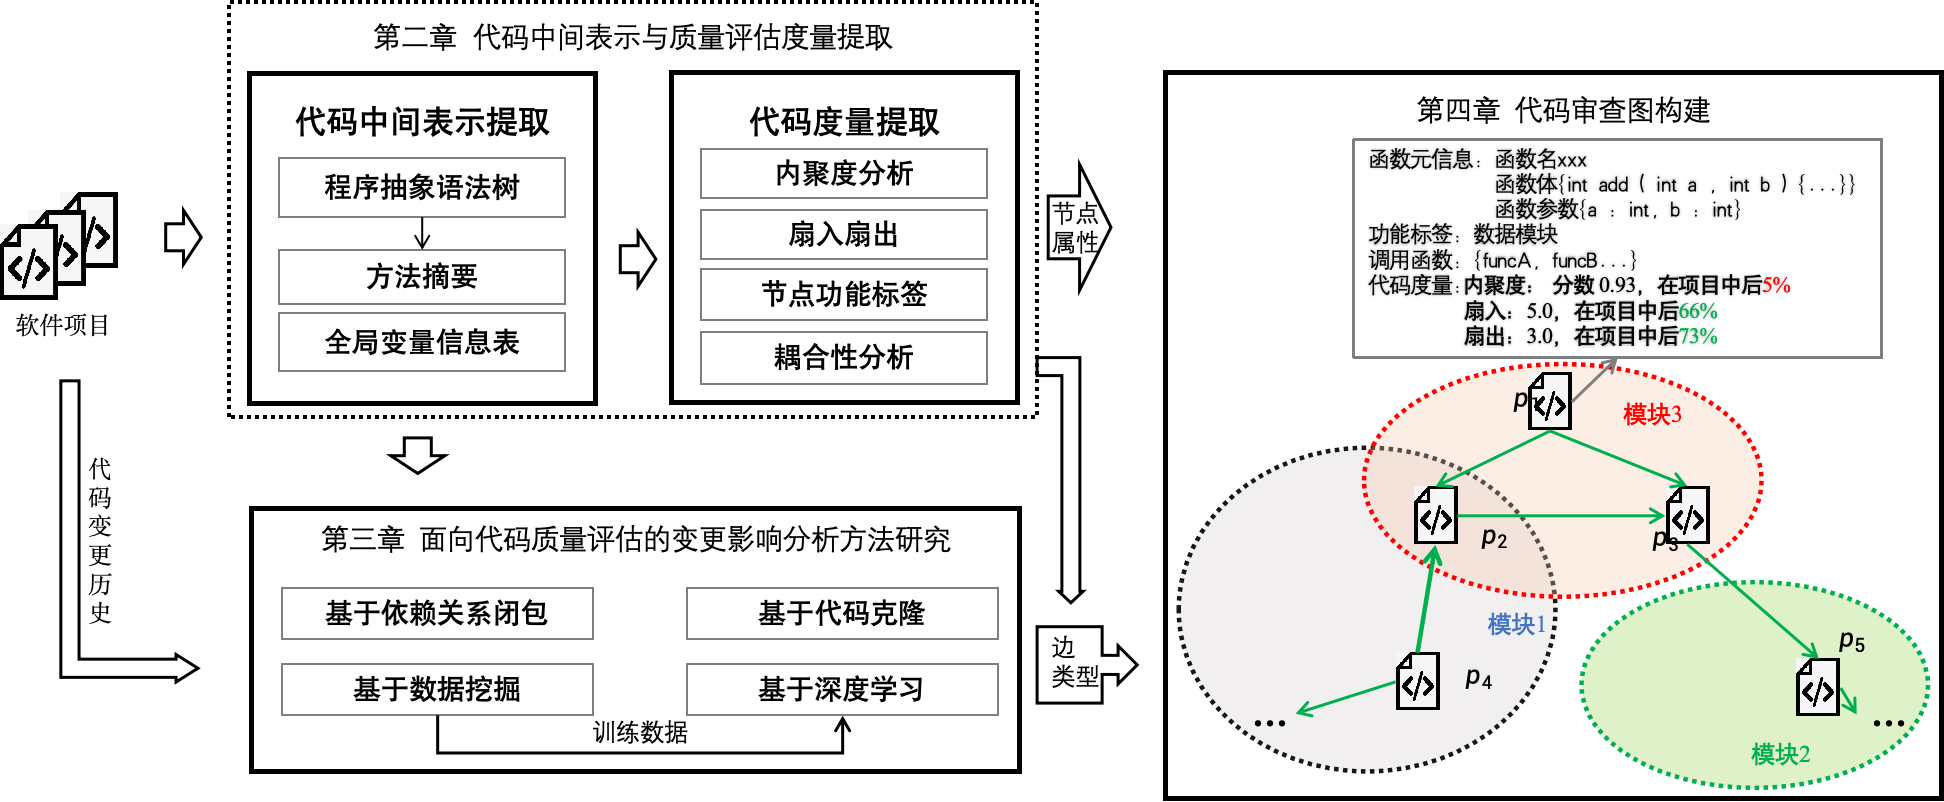
\includegraphics[width = 1.0\textwidth]{章节安排}
\caption{章节安排}
\end{figure}

第一章为绪论,首先介绍了本文的研究背景和研究现状,首先介绍了软件质量和代码变更影响的背景和意义,然后介绍了代码质量研究主题的国内外研究现状,介绍了代码质量度量套件的研究现状,并分别从静态和动态两类分析方法总结了变更影响分析的研究现状。然后介绍了本文的主要研究内容和章节安排。

第二章介绍了代码中间表示与质量评估度量提取。本章介绍了基于 clang 的抽象语法树生成方法,并且基于AST提取方法调用链和全局变量定义-使用链。基于提取的中间表示和特征,本章介绍了代码度量的提取,并进行了实验结果展示和分析。

第三章介绍了面向代码质量评估的变更影响分析方法研
究。分别介绍了基于依赖关系闭包的方法、基于代码克隆的方法、基于数据挖掘的方法和基于深度学习的方法。最后进行了实验结果展示和分析。

第四章介绍了代码审查图的生成。首先介绍了利用大语言模型生成模块标签,用于分析代码的模块化质量。其次介绍了代码审查图的构建方法,并通过图可视化引擎G6对图进行可视化,最后进行了实验结果展示和分析。



